% Options for packages loaded elsewhere
\PassOptionsToPackage{unicode}{hyperref}
\PassOptionsToPackage{hyphens}{url}
\documentclass[
  ignorenonframetext,
]{beamer}
\newif\ifbibliography
\usepackage{pgfpages}
\setbeamertemplate{caption}[numbered]
\setbeamertemplate{caption label separator}{: }
\setbeamercolor{caption name}{fg=normal text.fg}
\beamertemplatenavigationsymbolsempty
% remove section numbering
\setbeamertemplate{part page}{
  \centering
  \begin{beamercolorbox}[sep=16pt,center]{part title}
    \usebeamerfont{part title}\insertpart\par
  \end{beamercolorbox}
}
\setbeamertemplate{section page}{
  \centering
  \begin{beamercolorbox}[sep=12pt,center]{section title}
    \usebeamerfont{section title}\insertsection\par
  \end{beamercolorbox}
}
\setbeamertemplate{subsection page}{
  \centering
  \begin{beamercolorbox}[sep=8pt,center]{subsection title}
    \usebeamerfont{subsection title}\insertsubsection\par
  \end{beamercolorbox}
}
% Prevent slide breaks in the middle of a paragraph
\widowpenalties 1 10000
\raggedbottom
\AtBeginPart{
  \frame{\partpage}
}
\AtBeginSection{
  \ifbibliography
  \else
    \frame{\sectionpage}
  \fi
}
\AtBeginSubsection{
  \frame{\subsectionpage}
}
\usepackage{iftex}
\ifPDFTeX
  \usepackage[T1]{fontenc}
  \usepackage[utf8]{inputenc}
  \usepackage{textcomp} % provide euro and other symbols
\else % if luatex or xetex
  \usepackage{unicode-math} % this also loads fontspec
  \defaultfontfeatures{Scale=MatchLowercase}
  \defaultfontfeatures[\rmfamily]{Ligatures=TeX,Scale=1}
\fi
\usepackage{lmodern}
\ifPDFTeX\else
  % xetex/luatex font selection
\fi
% Use upquote if available, for straight quotes in verbatim environments
\IfFileExists{upquote.sty}{\usepackage{upquote}}{}
\IfFileExists{microtype.sty}{% use microtype if available
  \usepackage[]{microtype}
  \UseMicrotypeSet[protrusion]{basicmath} % disable protrusion for tt fonts
}{}
\makeatletter
\@ifundefined{KOMAClassName}{% if non-KOMA class
  \IfFileExists{parskip.sty}{%
    \usepackage{parskip}
  }{% else
    \setlength{\parindent}{0pt}
    \setlength{\parskip}{6pt plus 2pt minus 1pt}}
}{% if KOMA class
  \KOMAoptions{parskip=half}}
\makeatother
\usepackage{longtable,booktabs,array}
\usepackage{caption}
\captionsetup[table]{skip=6pt}
\newcounter{none} % for unnumbered tables
\usepackage{calc} % for calculating minipage widths
\usepackage{caption}
% Make caption package work with longtable
\makeatletter
\def\fnum@table{\tablename~\thetable}
\makeatother
\usepackage{graphicx}
\makeatletter
\newsavebox\pandoc@box
\newcommand*\pandocbounded[1]{% scales image to fit in text height/width
  \sbox\pandoc@box{#1}%
  \Gscale@div\@tempa{\textheight}{\dimexpr\ht\pandoc@box+\dp\pandoc@box\relax}%
  \Gscale@div\@tempb{\linewidth}{\wd\pandoc@box}%
  \ifdim\@tempb\p@<\@tempa\p@\let\@tempa\@tempb\fi% select the smaller of both
  \ifdim\@tempa\p@<\p@\scalebox{\@tempa}{\usebox\pandoc@box}%
  \else\usebox{\pandoc@box}%
  \fi%
}
% Set default figure placement to htbp
\def\fps@figure{htbp}
\makeatother
\setlength{\emergencystretch}{3em} % prevent overfull lines
\providecommand{\tightlist}{%
  \setlength{\itemsep}{0pt}\setlength{\parskip}{0pt}}
% Auto-generated by infrastructure/rendering/_pdf_latex_helpers.py::extract_math_font_preamble.
% Minimal header passed to Pandoc via -H so Beamer slides pick up the same math font
% as the combined-PDF path. Adjust the manuscript's preamble.md to change the font globally.
\usepackage{unicode-math}
\setmathfont{latinmodern-math.otf}

% Slide layout defaults for warning-clean scientific decks.
\usepackage{etoolbox}
\IfFileExists{xurl.sty}{\usepackage{xurl}}{}
\IfFileExists{seqsplit.sty}{\usepackage{seqsplit}}{\newcommand{\seqsplit}[1]{#1}}
\protected\def\breakseq#1{\seqsplit{#1}}
\protected\def\breaktt#1{\begingroup\ttfamily\seqsplit{#1}\endgroup}
\setlength{\emergencystretch}{6em}
\tolerance=5000
\hbadness=10000
\hfuzz=1pt
\setlength{\tabcolsep}{2pt}
\AtBeginEnvironment{longtable}{\tiny\renewcommand{\arraystretch}{0.86}\setlength{\tabcolsep}{1pt}}
\AtBeginEnvironment{tabular}{\tiny\renewcommand{\arraystretch}{0.86}\setlength{\tabcolsep}{1pt}}
\AtBeginEnvironment{equation}{\tiny}
\AtBeginEnvironment{equation*}{\tiny}
\AtBeginEnvironment{align}{\tiny}
\AtBeginEnvironment{align*}{\tiny}
\AtBeginEnvironment{itemize}{\footnotesize}
\AtBeginEnvironment{enumerate}{\footnotesize}
\AtBeginEnvironment{description}{\footnotesize}
\setbeamerfont{caption}{size=\tiny}
\setbeamerfont{caption name}{size=\tiny}
\setbeamerfont{normal text}{size=\small}
\setbeamerfont{frametitle}{size=\small}
\setbeamerfont{section title}{size=\footnotesize}
\setbeamerfont{subsection title}{size=\footnotesize}
\setbeamertemplate{section page}{%
  \centering
  \begin{beamercolorbox}[sep=12pt,center,wd=\paperwidth]{section title}
    \parbox{0.86\paperwidth}{\centering\usebeamerfont{section title}\insertsection\par}
  \end{beamercolorbox}
}
\setbeamertemplate{subsection page}{%
  \centering
  \begin{beamercolorbox}[sep=8pt,center,wd=\paperwidth]{subsection title}
    \parbox{0.86\paperwidth}{\centering\usebeamerfont{subsection title}\insertsubsection\par}
  \end{beamercolorbox}
}
\setlength{\abovecaptionskip}{2pt}
\setlength{\belowcaptionskip}{0pt}

% Natbib and cross-reference fallbacks — slides don't load natbib
% or cleveref, but combined-PDF manuscript prose may emit these
% commands. The fallback renders citations as a bracketed key list
% and cross-references as detokenized labels so slides don't fail on
% undefined control sequences or raw underscores. \providecommand is
% a no-op if packages load later.
\providecommand{\citep}[1]{[#1]}
\providecommand{\citet}[1]{#1}
\providecommand{\citealp}[1]{#1}
\providecommand{\citeauthor}[1]{#1}
\providecommand{\citeyear}[1]{#1}
\providecommand{\cref}[1]{\texttt{\detokenize{#1}}}
\providecommand{\Cref}[1]{\texttt{\detokenize{#1}}}

\newtheorem{proposition}{Proposition}
\newtheorem{hypothesis}{Hypothesis}
\usepackage{bookmark}
\IfFileExists{xurl.sty}{\usepackage{xurl}}{} % add URL line breaks if available
\urlstyle{same}
% fallback for those not using the hyperref driver hyperxmp:
\makeatletter
\@ifundefined{xmpquote}{\newcommand{\xmpquote}[1]{#1}}{}
\makeatother
\hypersetup{
  hidelinks,
  pdfcreator={LaTeX via pandoc}}

\author{\texorpdfstring{}{}}
\date{}

\begin{document}

\section{Supplement: Model-Bounded Variational and Expected Free Energy
Examples}\label{sec:supplement-vfe-efe}

\begin{frame}[allowframebreaks]{Supplement: Model-Bounded Variational
and Expected Free Energy Examples}
This supplement carries the kernel-level mathematical walkthroughs that
support the curriculum without crowding the main Results section. The
purpose is narrow: show how the claim registry, figures and prose
jointly teach the two optimization objectives that organize the course.
Variational free energy is used for belief updating under a fixed
generative model; expected free energy is used for policy evaluation
under uncertainty. Both examples are deliberately small enough to audit
by rerunning the kernels.

\end{frame}

\begin{frame}[allowframebreaks]{Supplement: Model-Bounded Variational
and Expected Free Energy Examples}
Notation is fixed before the examples: \(s\) is the latent state, \(o\)
is the observation, \(p(s)\) is the prior, \(p(o\mid s)\) is the
likelihood, \(p(o,s)\) is the joint generative density, and \(q(s)\) is
the recognition density. The variational free-energy convention is
\(F[q]=\mathbb{E}_{q(s)}[\ln q(s)-\ln p(o,s)]
=D_{\mathrm{KL}}(q(s)\|p(s\mid o))-\ln p(o)\), so the bound is tight
when \(q(s)\) equals the exact posterior. For expected free energy, this
supplement uses the lower-is-better policy convention
\(q(\pi)=\mathrm{softmax}(-\gamma G(\pi))\) with policy precision
\(\gamma\); the plotted terms are therefore tied to the stated policy
set and preference distribution, not to a universal sign convention
(Buckley et al. 2017; Parr et al. 2022; Millidge et al. 2021; Champion
et al. 2026; Nuijten, Lukashchuk, et al. 2026; Nuijten, Laar, et al.
2026).
\end{frame}

\subsection{SkillTree bridge from derivations to quiz-gated
subjects}\label{skilltree-bridge-from-derivations-to-quiz-gated-subjects}

\begin{frame}[fragile,allowframebreaks]{SkillTree bridge from
derivations to quiz-gated subjects}
The supplement is not an isolated appendix of equations. It is a bridge
from kernel claims to quiz-gated SkillTree material:
\texttt{sub\_free\_energy} and \texttt{sub\_efe} carry the core VFE/EFE
concepts, the scientific-supplement subjects train bound and term
interpretation, and the mastery subjects turn those interpretations into
route-handoff and quiz-authoring checks.
fig.~\ref{fig:vfe_efe_skilltree_bridge} is generated from the current
curriculum graph after structural checks and SkillTree route contract so
the text, figure, and dashboard artifact all point to the same subject,
skill, prerequisite-edge, quiz, and route data. This bridge also keeps
the VFE/EFE distinction scholarly rather than mnemonic: VFE is an
evidence bound for belief updating, while EFE is a policy-evaluation
objective whose formulations and preference assumptions need explicit
scope boundaries (Buckley et al. 2017; Parr et al. 2022; Smith et al.
2022; Millidge et al. 2021; Champion et al. 2026; Nuijten, Lukashchuk,
\end{frame}

\begin{frame}[fragile,allowframebreaks]{SkillTree bridge from
derivations to quiz-gated subjects}
et al. 2026; Nuijten, Laar, et al. 2026).

\end{frame}

\begin{frame}[fragile,allowframebreaks]{SkillTree bridge from
derivations to quiz-gated subjects}
{\def\LTcaptype{none} % do not increment counter
\begin{longtable}[]{@{}
  >{\raggedright\arraybackslash}p{(\linewidth - 14\tabcolsep) * \real{0.1111}}
  >{\raggedright\arraybackslash}p{(\linewidth - 14\tabcolsep) * \real{0.1111}}
  >{\raggedleft\arraybackslash}p{(\linewidth - 14\tabcolsep) * \real{0.1481}}
  >{\raggedleft\arraybackslash}p{(\linewidth - 14\tabcolsep) * \real{0.1481}}
  >{\raggedleft\arraybackslash}p{(\linewidth - 14\tabcolsep) * \real{0.1481}}
  >{\raggedright\arraybackslash}p{(\linewidth - 14\tabcolsep) * \real{0.1111}}
  >{\raggedright\arraybackslash}p{(\linewidth - 14\tabcolsep) * \real{0.1111}}
  >{\raggedright\arraybackslash}p{(\linewidth - 14\tabcolsep) * \real{0.1111}}@{}}
\toprule\noalign{}
\begin{minipage}[b]{\linewidth}\raggedright
Layer
\end{minipage} & \begin{minipage}[b]{\linewidth}\raggedright
Skills
\end{minipage} & \begin{minipage}[b]{\linewidth}\raggedleft
Prerequisite edges
\end{minipage} & \begin{minipage}[b]{\linewidth}\raggedleft
Depth
\end{minipage} & \begin{minipage}[b]{\linewidth}\raggedleft
Representative IDs
\end{minipage} & \begin{minipage}[b]{\linewidth}\raggedright
Learn route
\end{minipage} & \begin{minipage}[b]{\linewidth}\raggedright
Quiz route
\end{minipage} & \begin{minipage}[b]{\linewidth}\raggedright
\end{minipage} \\
\midrule\noalign{}
\endhead
VFE core & 7 & 16 total; 6 internal & 7-10 &
\texttt{vm\_elbo}\breaktt{vm\_perception\_descent}\breaktt{vm\_message\_passing}
& \breaktt{/subjects/sub\_free\_energy} &
\breaktt{/subjects/sub\_free\_energy/skills/vm\_message\_passing/quizzes/vm\_message\_passing\_quiz}
& \\
EFE core & 7 & 15 total; 7 internal & 18-20 &
\breaktt{ai\_expected\_free\_energy}\breaktt{ai\_explore\_exploit}\breaktt{ai\_free\_energy\_of\_future}
& \breaktt{/subjects/sub\_efe} &
\breaktt{/subjects/sub\_efe/skills/ai\_free\_energy\_of\_future/quizzes/ai\_free\_energy\_of\_future\_quiz}
& \\
VFE supplement & 6 & 11 total; 5 internal & 9-14 &
\breaktt{sci\_variational\_01}\breaktt{sci\_variational\_04}\breaktt{sci\_variational\_06}
& \breaktt{/subjects/sub\_scientific\_supplement\_variational} &
\breaktt{/subjects/sub\_scientific\_supplement\_variational/skills/sci\_variational\_06/quizzes/sci\_variational\_06\_quiz}
& \\
EFE supplement & 6 & 11 total; 5 internal & 19-24 &
\breaktt{sci\_active\_inference\_01}\breaktt{sci\_active\_inference\_04}\breaktt{sci\_active\_inference\_06}
& \breaktt{/subjects/sub\_scientific\_supplement\_active\_inference} &
\breaktt{/subjects/sub\_scientific\_supplement\_active\_inference/skills/sci\_active\_inference\_06/quizzes/sci\_active\_inference\_06\_quiz}
& \\
VFE mastery & 8 & 17 total; 7 internal & 36-43 &
\breaktt{mastery\_variational\_01}\breaktt{mastery\_variational\_05}\breaktt{mastery\_variational\_08}
& \breaktt{/subjects/sub\_skilltree\_mastery\_variational} &
\breaktt{/subjects/sub\_skilltree\_mastery\_variational/skills/mastery\_variational\_08/quizzes/mastery\_variational\_08\_quiz}
& \\
EFE mastery & 8 & 17 total; 7 internal & 52-59 &
\breaktt{mastery\_active\_inference\_01}\breaktt{mastery\_active\_inference\_05}\breaktt{mastery\_active\_inference\_08}
& \breaktt{/subjects/sub\_skilltree\_mastery\_active\_inference} &
\breaktt{/subjects/sub\_skilltree\_mastery\_active\_inference/skills/mastery\_active\_inference\_08/quizzes/mastery\_active\_inference\_08\_quiz}
& \\
\bottomrule\noalign{}
\end{longtable}
}
\end{frame}

\begin{frame}[allowframebreaks]{Bridge figure}
\protect\phantomsection\label{bridge-figure}
\end{frame}

\begin{frame}[allowframebreaks]{Bridge figure}
\begin{figure}
\centering
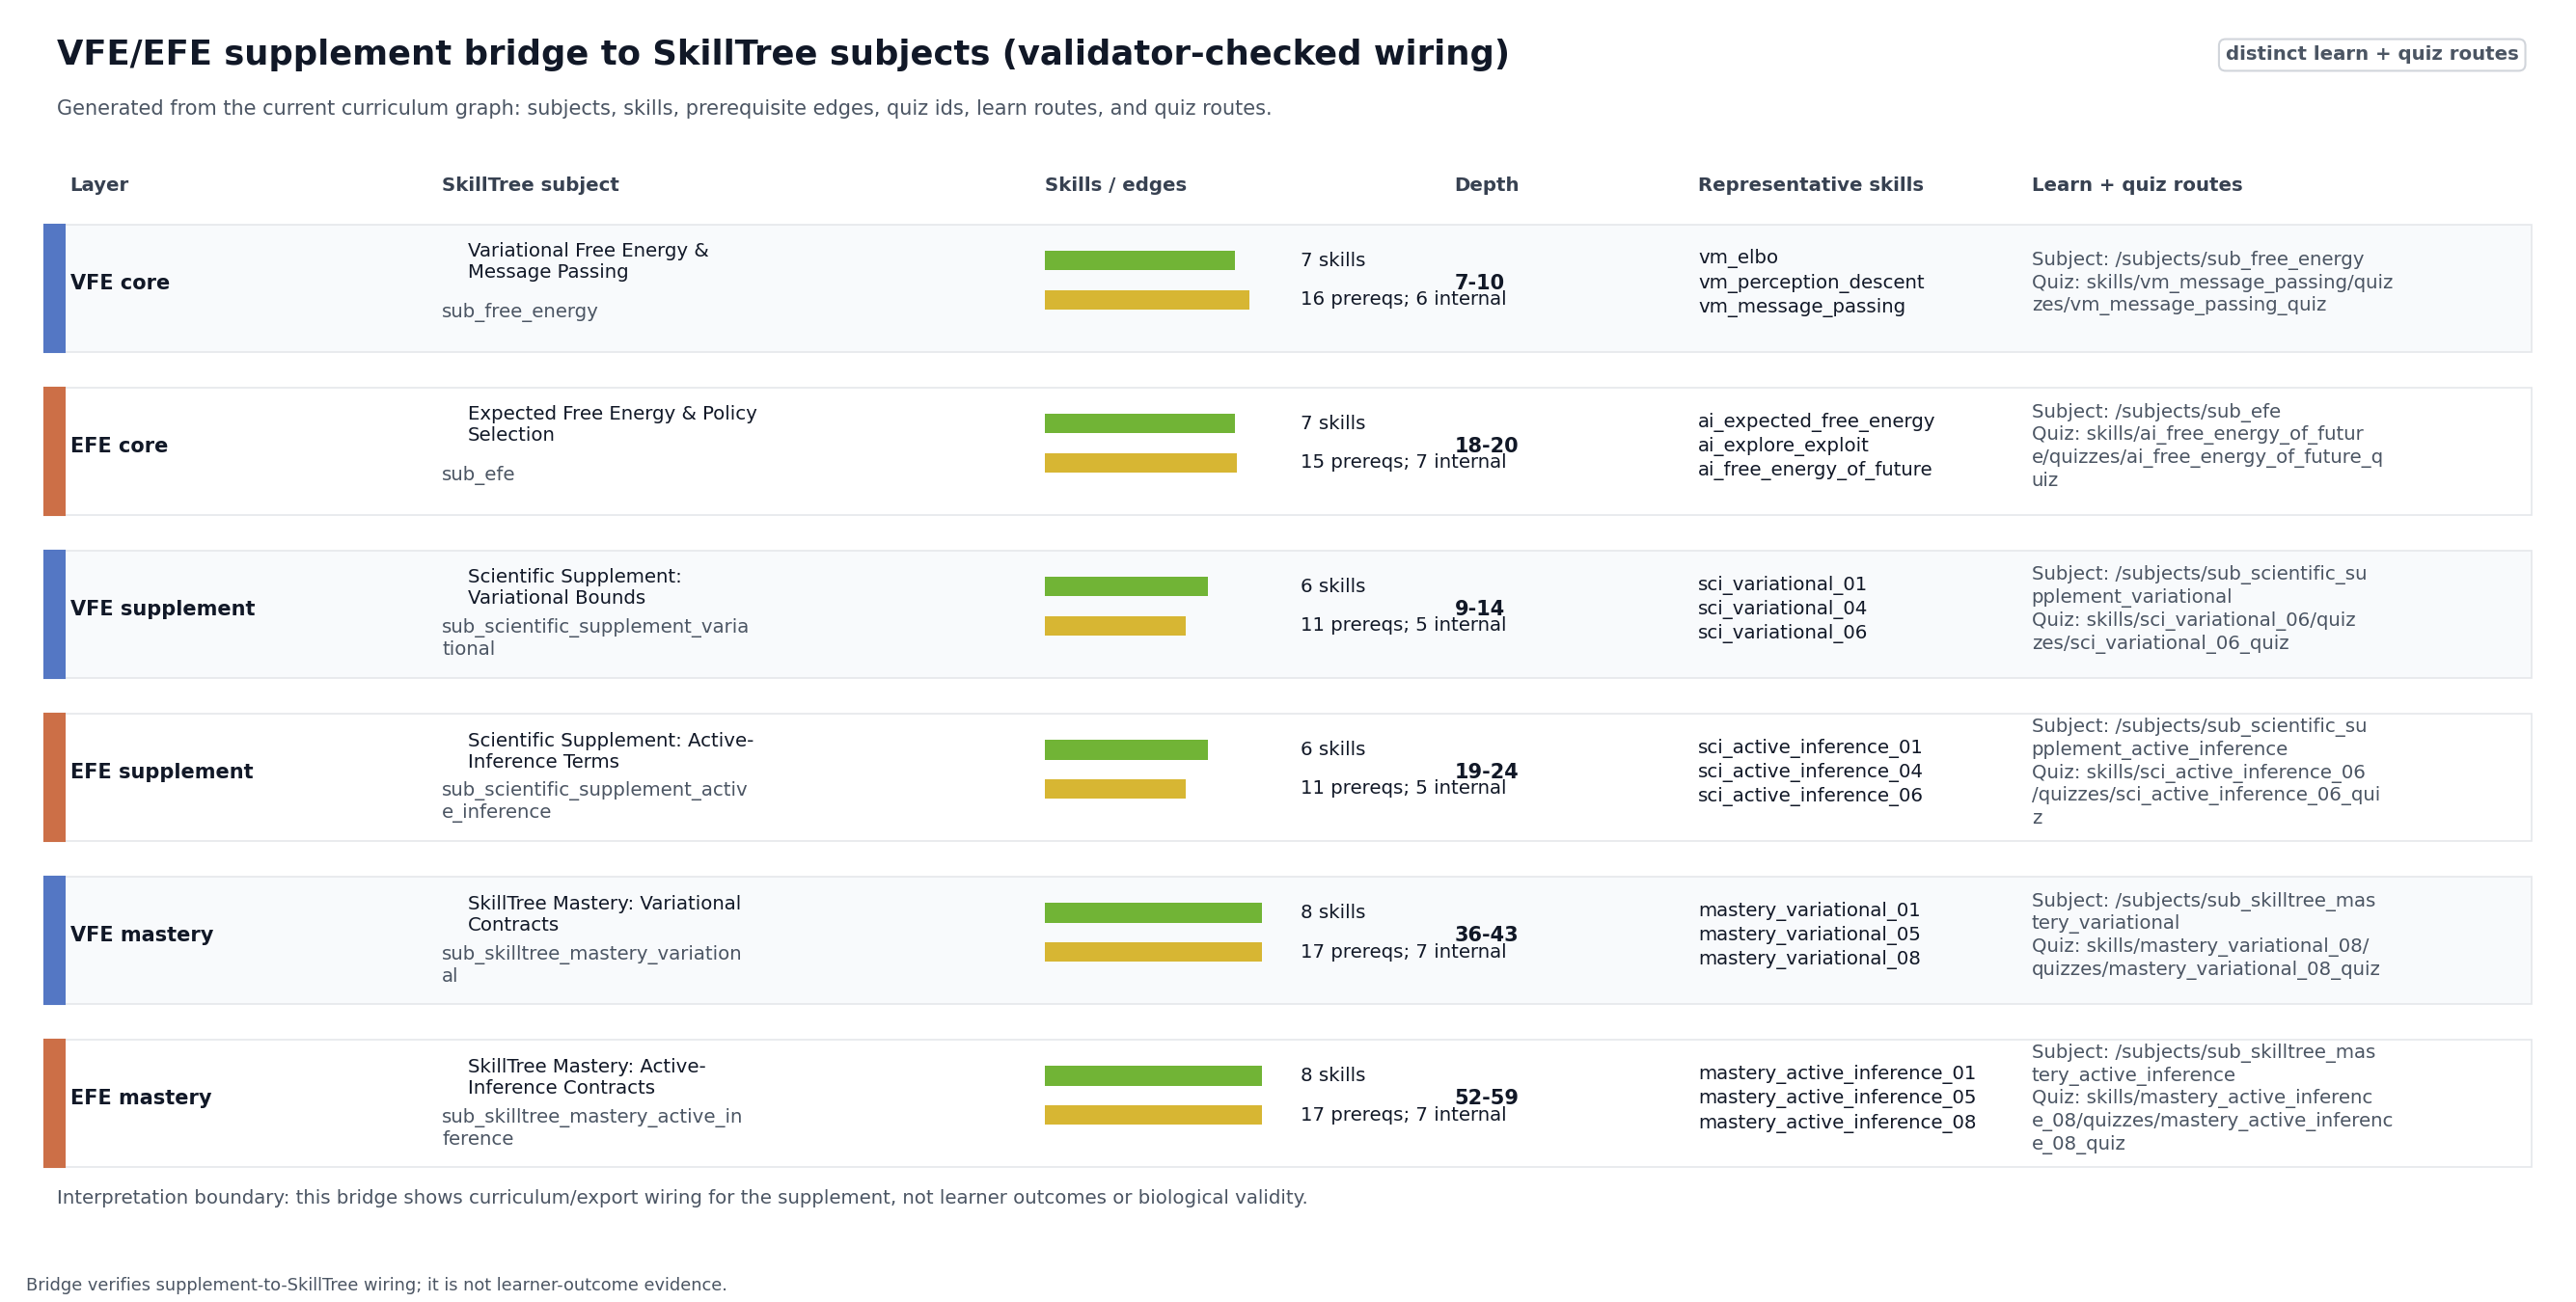
\includegraphics[width=1\linewidth,height=0.40\textheight,keepaspectratio,alt={VFE/EFE SkillTree bridge generated from the current curriculum graph after structural checks. Rows are real SkillTree subjects, columns report skill counts, prerequisite-edge counts, graph-depth ranges, representative skill IDs, and learn-route and quiz-route fragments that expose the subject identifiers; color marks separate VFE-centered rows from EFE-centered rows. The figure connects the supplement's mathematical plots to quiz-gated curriculum nodes and prevents the derivation from being presented as a standalone artifact disconnected from the learning path.}]{../figures/vfe_efe_skilltree_bridge.png}
\caption{VFE/EFE SkillTree bridge generated from the current curriculum
graph after structural checks. Rows are real SkillTree subjects, columns
report skill counts, prerequisite-edge counts, graph-depth ranges,
representative skill IDs, and learn-route and quiz-route fragments that
expose the subject identifiers; color marks separate VFE-centered rows
from EFE-centered rows. The figure connects the supplement's
mathematical plots to quiz-gated curriculum nodes and prevents the
derivation from being presented as a standalone artifact disconnected
from the learning path.}\label{fig:vfe_efe_skilltree_bridge}
\end{figure}
\end{frame}

\subsection{Noisy-sensor posterior and the tight variational-free-energy
bound}\label{noisy-sensor-posterior-and-the-tight-variational-free-energy-bound}

\begin{frame}[fragile,allowframebreaks]{Noisy-sensor posterior and the
tight variational-free-energy bound}
On a noisy-sensor model with a \(1\%\) base rate, \(99\%\) sensitivity,
and \(95\%\) specificity, a positive observation yields a posterior of
0.166667 for the latent condition. This is the same base-rate
calibration problem that makes Bayesian reasoning difficult in
natural-language judgment tasks and motivates frequency-format teaching
examples for Bayesian inference (Cosmides and Tooby 1996; Gigerenzer and
Hoffrage 1995). The evidence probability of the positive observation is
0.0594, so the observation surprise is 2.82346 nats.

\end{frame}

\begin{frame}[fragile,allowframebreaks]{Noisy-sensor posterior and the
tight variational-free-energy bound}
{\def\LTcaptype{none} % do not increment counter
\begin{longtable}[]{@{}
  >{\raggedright\arraybackslash}p{(\linewidth - 2\tabcolsep) * \real{0.5000}}
  >{\raggedright\arraybackslash}p{(\linewidth - 2\tabcolsep) * \real{0.5000}}@{}}
\toprule\noalign{}
\begin{minipage}[b]{\linewidth}\raggedright
Noisy-sensor parameter
\end{minipage} & \begin{minipage}[b]{\linewidth}\raggedright
Paper value
\end{minipage} \\
\midrule\noalign{}
\endhead
Latent states & \texttt{present}, \texttt{absent} \\
Observation index & \texttt{positive} \\
Prior \(D\) & \([0.01, 0.99]\) \\
Likelihood rows \(A_{o,s}\) & \texttt{positive}: \([0.99, 0.05]\);
\texttt{negative}: \([0.01, 0.95]\) \\
VFE sweep coordinate & \(q(\mathrm{present})\) over \([0.001, 0.999]\),
plus the exact posterior and \(0.5\) \\
\bottomrule\noalign{}
\end{longtable}
}

\end{frame}

\begin{frame}[fragile,allowframebreaks]{Noisy-sensor posterior and the
tight variational-free-energy bound}
Evaluating variational free energy across beliefs confirms the central
inequality: a uniform belief gives 3.11735 nats, while the true
posterior gives 2.82346 nats, exactly the negative log-evidence.
fig.~\ref{fig:free_energy} shows the full one-dimensional sweep over
\(q(\mathrm{present})\): the curve bottoms out at the exact posterior
and stays above the surprise line everywhere else. The plot should not
be read as a universal geometry of all recognition densities. It is a
controlled diagnostic for one discrete model, one observation and one
belief coordinate.

\end{frame}

\begin{frame}[fragile,allowframebreaks]{Noisy-sensor posterior and the
tight variational-free-energy bound}
\begin{figure}
\centering
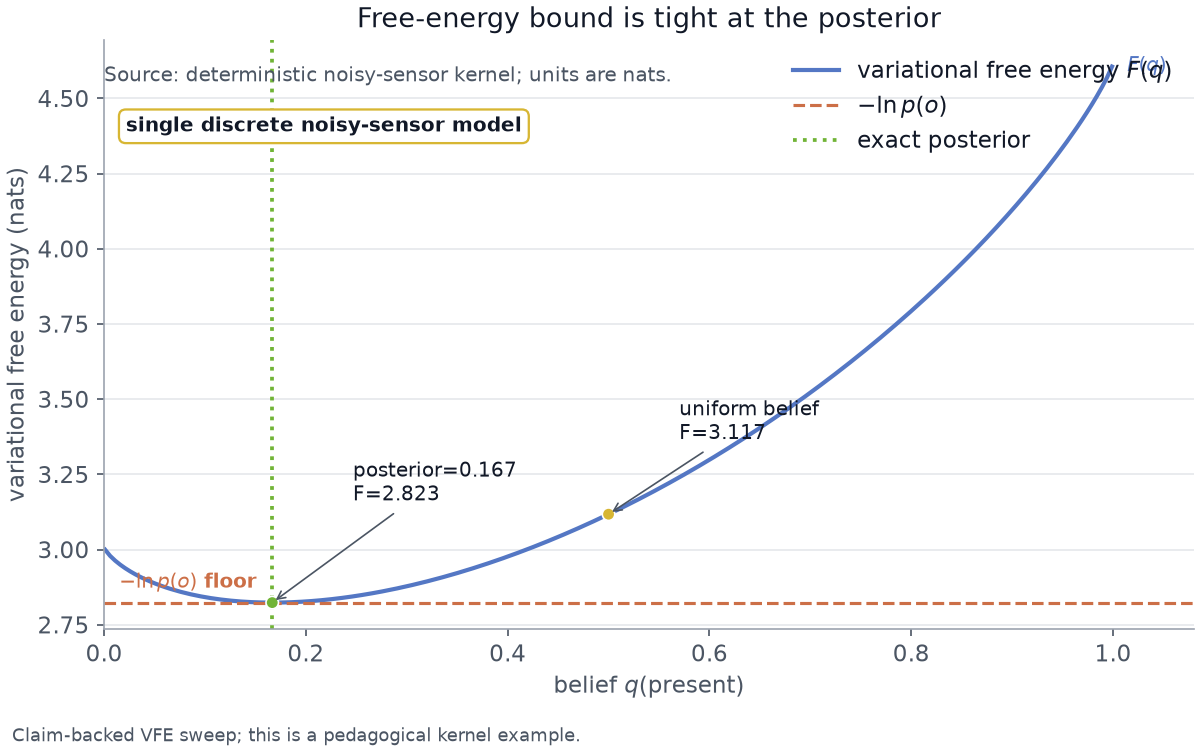
\includegraphics[width=1\linewidth,height=0.40\textheight,keepaspectratio,alt={Variational free-energy sweep for the noisy-sensor model, generated from the same claim-registry kernels that provide the manuscript tokens and taught through the VFE core, supplement, and mastery SkillTree subjects in the VFE/EFE SkillTree bridge. The x-axis is the recognition belief q(\textbackslash mathrm\{present\}), the blue curve is F(q) in nats, the horizontal dashed line is -\textbackslash ln p(o), the vertical dotted line is the exact posterior, and the labeled points compare the looser uniform belief with the posterior value. The intended takeaway is bound tightness at the posterior for this one discrete model and observation; the plot does not establish that the model is true or that the same geometry holds for every recognition family.}]{../figures/free_energy_descent.png}
\caption{Variational free-energy sweep for the noisy-sensor model,
generated from the same claim-registry kernels that provide the
manuscript tokens and taught through the VFE core, supplement, and
mastery SkillTree subjects in the VFE/EFE SkillTree bridge. The x-axis
is the recognition belief \(q(\mathrm{present})\), the blue curve is
\(F(q)\) in nats, the horizontal dashed line is \(-\ln p(o)\), the
vertical dotted line is the exact posterior, and the labeled points
compare the looser uniform belief with the posterior value. The intended
takeaway is bound tightness at the posterior for this one discrete model
and observation; the plot does not establish that the model is true or
that the same geometry holds for every recognition
family.}\label{fig:free_energy}
\end{figure}
\end{frame}

\subsection{Expected free energy: epistemic value and bounded policy
comparison}\label{expected-free-energy-epistemic-value-and-bounded-policy-comparison}

\begin{frame}[allowframebreaks]{Expected free energy: epistemic value
and bounded policy comparison}
Decomposing expected free energy on an informative sensor shows that an
uncertain belief carries positive epistemic value (0.368064 nats) while
a certain belief carries none (0 nats): once the state is known, an
observation cannot reduce uncertainty. In the two-action agent,
preferences are neutral, so the pragmatic term is identical for both
actions and the choice is decided by information gain. Under the
lower-is-better \(G(\pi)\) convention above, the information-seeking
\emph{sample} action scores lower expected free energy (0.546837 nats)
than \emph{commit} (0.613267 nats), because it carries higher epistemic
value (0.146311 nats versus 0.079881 nats). This is the epistemic drive
of Active Inference: no separate curiosity bonus is required in the
reference formulation used here (Friston et al. 2015, 2017; Da Costa et
al. 2020; Sajid et al. 2021). Derivation and unification work is the
\end{frame}

\begin{frame}[allowframebreaks]{Expected free energy: epistemic value
and bounded policy comparison}
reason the supplement keeps the formulation explicit instead of
presenting ``expected free energy'' as a single unqualified object
(Millidge et al. 2021; Champion et al. 2026; Nuijten, Lukashchuk, et al.
2026; Nuijten, Laar, et al. 2026).
\end{frame}

\begin{frame}[fragile,allowframebreaks]{Preference convention and
parameters}
\protect\phantomsection\label{preference-convention-and-parameters}
One convention should be made explicit here: the kernel normalizes the
preference vector \(C\) to a probability distribution before taking its
logarithm for the pragmatic term (\breaktt{preferences\ =\ normalize(C)},
then \(\mathbb{E}_{q(o)}[\ln \mathrm{normalize}(C)]\)), so the values
plotted above assume \(C\) is a preference \emph{distribution}. This is
a specific modeling choice rather than the only option: canonical Active
Inference often treats \(C\) directly as a vector of log-preferences,
which shifts the pragmatic term by an additive constant and can change
its scale relative to the epistemic term.
\end{frame}

\begin{frame}[fragile,allowframebreaks]{EFE parameter table}
\protect\phantomsection\label{efe-parameter-table}
\end{frame}

\begin{frame}[fragile,allowframebreaks]{EFE parameter table}
{\def\LTcaptype{none} % do not increment counter
\begin{longtable}[]{@{}
  >{\raggedright\arraybackslash}p{(\linewidth - 2\tabcolsep) * \real{0.5000}}
  >{\raggedright\arraybackslash}p{(\linewidth - 2\tabcolsep) * \real{0.5000}}@{}}
\toprule\noalign{}
\begin{minipage}[b]{\linewidth}\raggedright
EFE sample/commit parameter
\end{minipage} & \begin{minipage}[b]{\linewidth}\raggedright
Paper value
\end{minipage} \\
\midrule\noalign{}
\endhead
Sensor likelihood & \(A=[[p,1-p],[1-p,p]]\), with \(p=0.9\) \\
EFE decomposition preference & \(C=[0.9,0.1]\) for the
informative-sensor term example \\
Agent preference & Neutral \(C=[0.5,0.5]\) for the sample/commit policy
comparison \\
Prior before observation & \(D=[0.5,0.5]\) \\
Actions & \texttt{sample} uses identity dynamics; \texttt{commit} maps
both prior states toward state \texttt{0} with transition columns
\([0.95,0.05]\) \\
Policy posterior & \(q(\pi)=\mathrm{softmax}(-\gamma G_\pi)\) over the
two one-step policies \\
\bottomrule\noalign{}
\end{longtable}
}
\end{frame}

\subsection{Sensor precision as a sample-versus-commit policy
boundary}\label{sensor-precision-as-a-sample-versus-commit-policy-boundary}

\begin{frame}[allowframebreaks]{Sensor precision as a
sample-versus-commit policy boundary}
The expected-free-energy result is not a universal law. It is pinned to
a specific moderate-precision regime: at sensor precision \(0.9\),
sampling wins; at the computed switch precision 0.95, sample and commit
tie; above that point, the commit action can become lower in expected
free energy. fig.~\ref{fig:efe} shows both the sample/commit comparison
and the precision sweep, making the regime boundary explicit instead of
hiding it in prose (Millidge et al. 2021; Champion et al. 2026; Nuijten,
Lukashchuk, et al. 2026; Nuijten, Laar, et al. 2026).

\end{frame}

\begin{frame}[allowframebreaks]{Sensor precision as a
sample-versus-commit policy boundary}
{\def\LTcaptype{none} % do not increment counter
\begin{longtable}[]{@{}
  >{\raggedright\arraybackslash}p{(\linewidth - 2\tabcolsep) * \real{0.5000}}
  >{\raggedright\arraybackslash}p{(\linewidth - 2\tabcolsep) * \real{0.5000}}@{}}
\toprule\noalign{}
\begin{minipage}[b]{\linewidth}\raggedright
Precision-sweep parameter
\end{minipage} & \begin{minipage}[b]{\linewidth}\raggedright
Paper value
\end{minipage} \\
\midrule\noalign{}
\endhead
Sensor precision range & \(p \in [0.5,0.99]\) with the computed switch
inserted into the grid \\
Sweep samples & \(101\) grid samples before inserting \(p=0.9\) and the
switch precision \\
Prior, preference, actions & Same neutral two-action agent as the
sample/commit comparison \\
Tie criterion & The switch is the bisection point where
\(G_{\mathrm{sample}}-G_{\mathrm{commit}}=0\) \\
\bottomrule\noalign{}
\end{longtable}
}

\begin{figure}
\centering
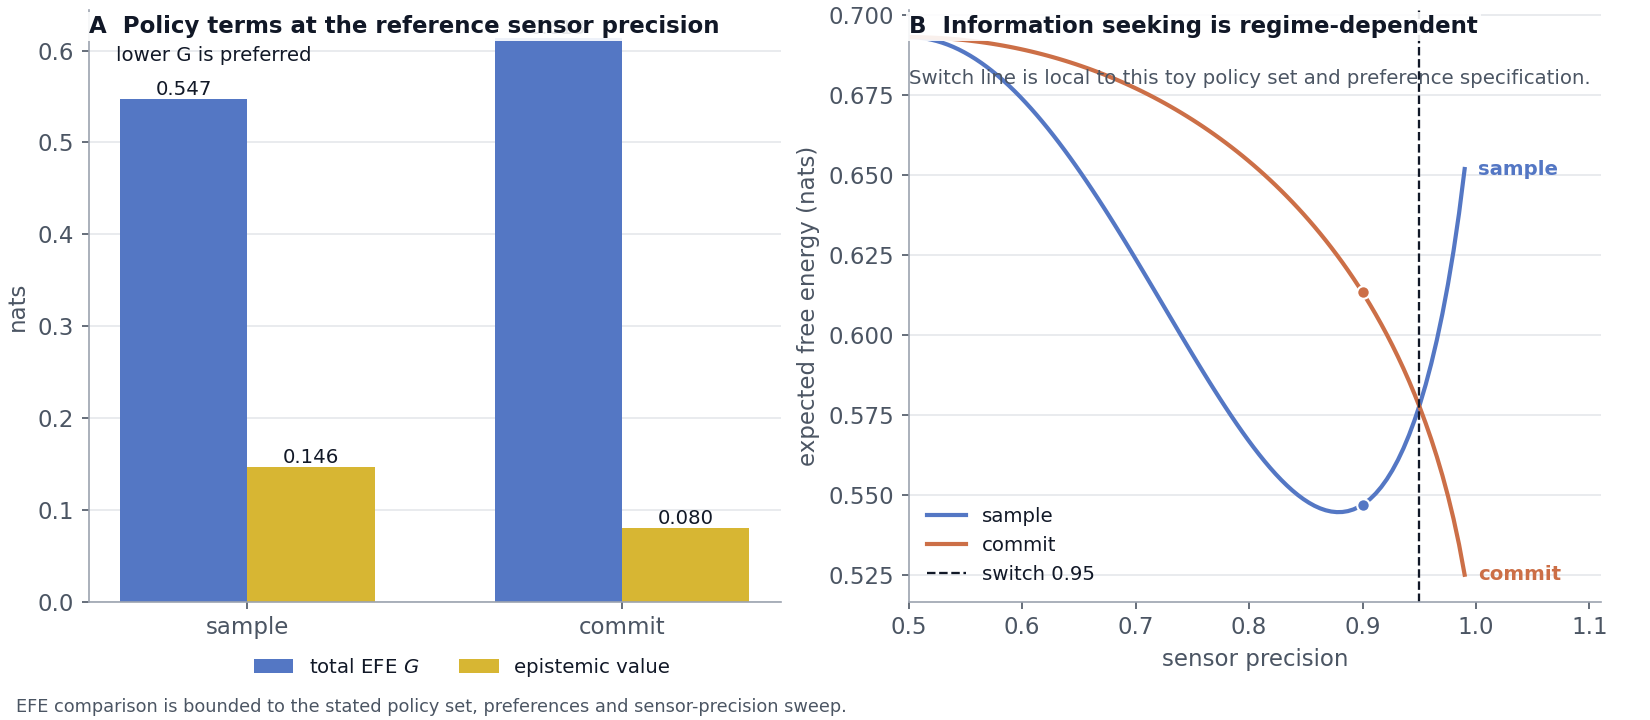
\includegraphics[width=1\linewidth,height=0.40\textheight,keepaspectratio,alt={Expected free-energy decomposition for the sample/commit task, generated from the discrete active-inference kernel and taught through the EFE core, supplement, and mastery SkillTree subjects in the VFE/EFE SkillTree bridge. The left panel compares total expected free energy and epistemic value for the two policies at sensor precision 0.9; the right panel sweeps sensor precision and marks the computed sample/commit switch. The visual encoding keeps policy score and epistemic value separate so the reader can see why sampling is preferred in the reference regime, while the right panel prevents the teaching example from being overgeneralized beyond the stated policy set and preferences.}]{../figures/efe_decomposition.png}
\caption{Expected free-energy decomposition for the sample/commit task,
generated from the discrete active-inference kernel and taught through
the EFE core, supplement, and mastery SkillTree subjects in the VFE/EFE
SkillTree bridge. The left panel compares total expected free energy and
epistemic value for the two policies at sensor precision \(0.9\); the
right panel sweeps sensor precision and marks the computed sample/commit
switch. The visual encoding keeps policy score and epistemic value
separate so the reader can see why sampling is preferred in the
reference regime, while the right panel prevents the teaching example
from being overgeneralized beyond the stated policy set and
preferences.}\label{fig:efe}
\end{figure}

\end{frame}

\begin{frame}[allowframebreaks]{Sensor precision as a
sample-versus-commit policy boundary}
fig.~\ref{fig:kernel_sensitivity_profiles} broadens the sensitivity view
without changing the evidence class. The left panel varies the base rate
in the same noisy-sensor likelihood and shows how a positive
observation's posterior changes as the prior changes. The middle panel
repeats the VFE bound profile so the equality point remains tied to the
exact posterior. The right panel repeats the EFE precision sweep and
marks the computed sample/commit boundary. These panels are
deterministic kernel diagnostics: they identify where the teaching
example is stable or regime-limited, not whether a learner or a
biological system will behave that way.

\end{frame}

\begin{frame}[allowframebreaks]{Sensor precision as a
sample-versus-commit policy boundary}
\begin{figure}
\centering
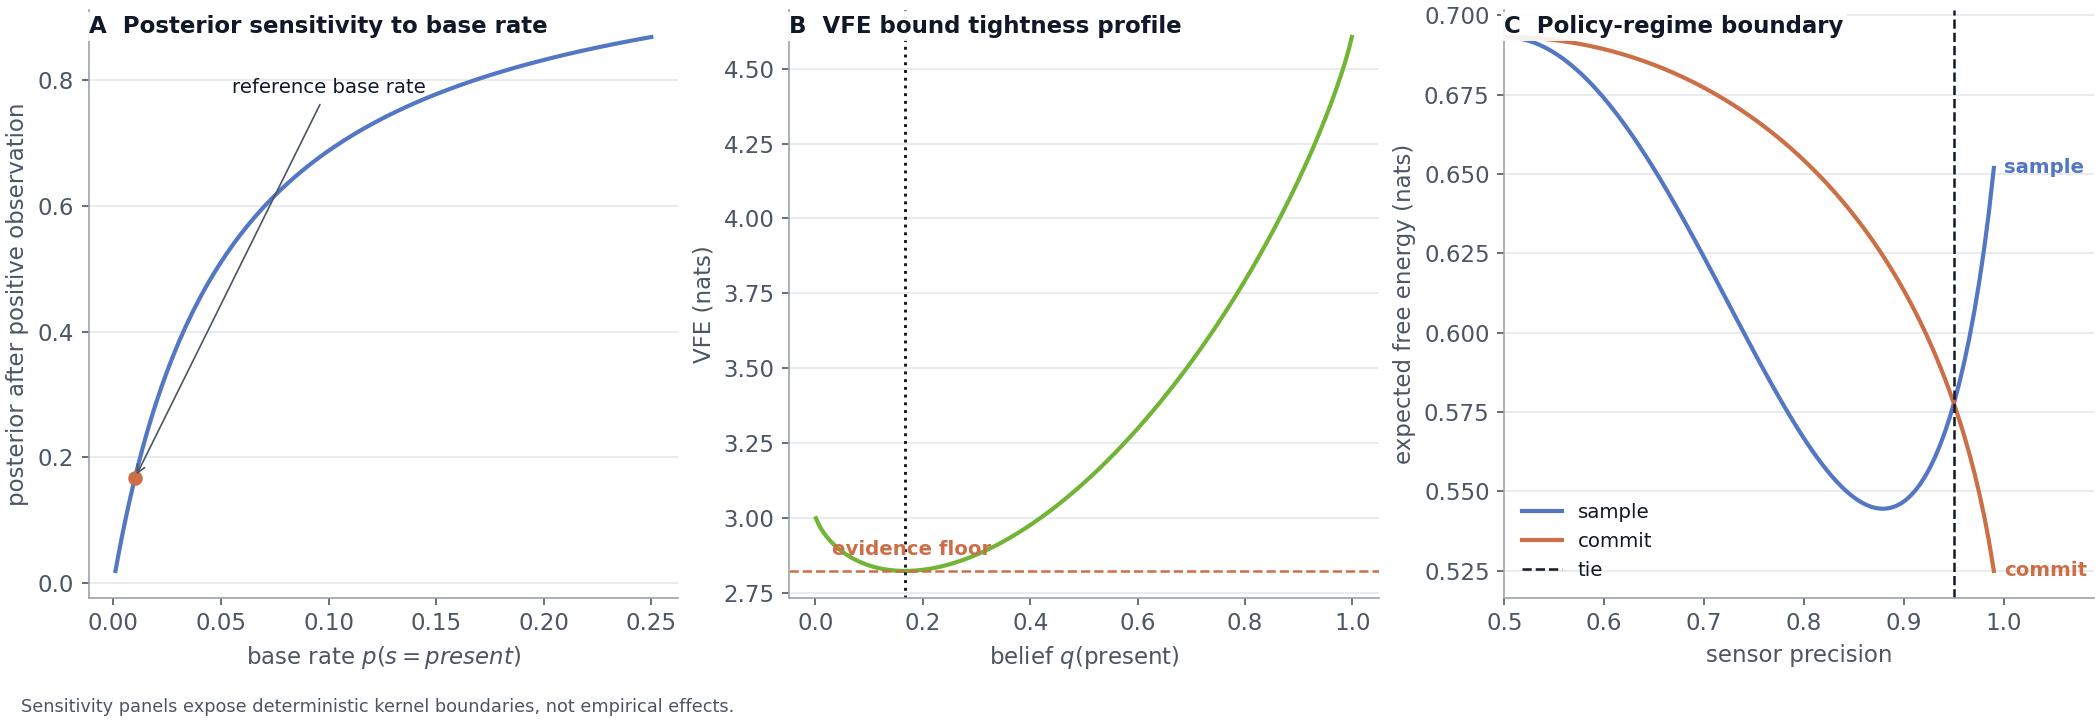
\includegraphics[width=1\linewidth,height=0.40\textheight,keepaspectratio,alt={Kernel sensitivity profiles for the supplemental examples, generated from the noisy-sensor posterior, VFE sweep, and EFE precision sweep, then positioned in the SkillTree bridge as a route from mathematical identity to quiz-gated interpretation. The left panel varies the base rate and shows posterior sensitivity after a positive observation, the middle panel plots the VFE bound profile with posterior and evidence references, and the right panel sweeps expected free energy for sample and commit policies across sensor precision while marking the computed policy switch. These panels identify deterministic regime boundaries for teaching examples; they are not empirical estimates, confidence intervals, or learner outcome statistics.}]{../figures/kernel_sensitivity_profiles.png}
\caption{Kernel sensitivity profiles for the supplemental examples,
generated from the noisy-sensor posterior, VFE sweep, and EFE precision
sweep, then positioned in the SkillTree bridge as a route from
mathematical identity to quiz-gated interpretation. The left panel
varies the base rate and shows posterior sensitivity after a positive
observation, the middle panel plots the VFE bound profile with posterior
and evidence references, and the right panel sweeps expected free energy
for sample and commit policies across sensor precision while marking the
computed policy switch. These panels identify deterministic regime
boundaries for teaching examples; they are not empirical estimates,
confidence intervals, or learner outcome
statistics.}\label{fig:kernel_sensitivity_profiles}
\end{figure}
\end{frame}

\subsection{Exact inference on a chain with sum-product belief
propagation}\label{exact-inference-on-a-chain-with-sum-product-belief-propagation}

\begin{frame}[allowframebreaks]{Exact inference on a chain with
sum-product belief propagation}
The message-passing curriculum is bound to a worked example rather than
left as prose. Because the example factor graph is acyclic, sum-product
belief propagation returns the exact node marginals for a three-node
sticky latent chain with a single informative reading at the middle
node. The observed node settles at 0.9, and the smoothing message lifts
each unobserved neighbor from its prior to 0.74 -- a lift of 0.24 that
is produced purely by propagating the one reading along the transition
factor. Because a chain is a tree, these marginals are the same numbers
a brute-force enumeration of the full joint would give; the test suite
pins that equality, so the example is an exact-inference check, not an
approximation (Kschischang et al. 2001; Pearl 1988; Parr et al. 2022).
Factor-graph message passing is also a live implementation path for EFE
minimization, but this supplement uses the chain only to teach exact
\end{frame}

\begin{frame}[allowframebreaks]{Exact inference on a chain with
sum-product belief propagation}
sum-product inference and keeps policy-optimization message passing out
of scope for this release (Nuijten et al. 2025).
\end{frame}

\begin{frame}[allowframebreaks]{Sum-product parameter table}
\protect\phantomsection\label{sum-product-parameter-table}
\end{frame}

\begin{frame}[allowframebreaks]{Sum-product parameter table}
{\def\LTcaptype{none} % do not increment counter
\begin{longtable}[]{@{}
  >{\raggedright\arraybackslash}p{(\linewidth - 2\tabcolsep) * \real{0.5000}}
  >{\raggedright\arraybackslash}p{(\linewidth - 2\tabcolsep) * \real{0.5000}}@{}}
\toprule\noalign{}
\begin{minipage}[b]{\linewidth}\raggedright
Sum-product parameter
\end{minipage} & \begin{minipage}[b]{\linewidth}\raggedright
Paper value
\end{minipage} \\
\midrule\noalign{}
\endhead
Chain length & \(3\) binary latent nodes \\
Prior on node \(0\) & \([0.5,0.5]\) \\
Sticky transition & \([[0.8,0.2],[0.2,0.8]]\) \\
Evidence potentials & node \(0\): \([1,1]\); node \(1\): \([0.9,0.1]\);
node \(2\): \([1,1]\) \\
\bottomrule\noalign{}
\end{longtable}
}
\end{frame}

\subsection{Conjugate parameter learning from Dirichlet
beliefs}\label{conjugate-parameter-learning-from-dirichlet-beliefs}

\begin{frame}[allowframebreaks]{Conjugate parameter learning from
Dirichlet beliefs}
Parameter learning is shown as a Dirichlet-conjugate update of one
sensor column. A flat prior has mean 0.5; after a fixed observed count
vector the posterior mean sharpens to 0.75, and the expected
log-parameter that variational message passing actually consumes is
-0.30202 nats, computed through the digamma identity
\(\mathbb{E}[\ln p_i]=\psi(\alpha_i)-\psi(\sum_j\alpha_j)\). This is the
learning half of active inference: beliefs about model parameters move
with evidence, not just beliefs about states (Da Costa et al. 2020).
\end{frame}

\subsection{Bayesian model reduction: whether data require added
structure}\label{bayesian-model-reduction-whether-data-require-added-structure}

\begin{frame}[fragile,allowframebreaks]{Bayesian model reduction:
whether data require added structure}
Bayesian model reduction compares the evidence of a full model against a
reduced model whose pruned state carries negligible prior mass. After a
positive reading on the noisy-sensor model the full-model log evidence
is -2.82346 nats and the reduced-model log evidence is -2.99571 nats, so
the log Bayes factor is 0.172252 nats. The positive sign says the data
support keeping the pruned structure: the reduced model is rejected.
Both terms are exact log evidences, so the reported factor is the
difference of two computed numbers rather than a hand-typed value
(Friston et al. 2018; Parr et al. 2022).

\end{frame}

\begin{frame}[fragile,allowframebreaks]{Bayesian model reduction:
whether data require added structure}
{\def\LTcaptype{none} % do not increment counter
\begin{longtable}[]{@{}
  >{\raggedright\arraybackslash}p{(\linewidth - 2\tabcolsep) * \real{0.5000}}
  >{\raggedright\arraybackslash}p{(\linewidth - 2\tabcolsep) * \real{0.5000}}@{}}
\toprule\noalign{}
\begin{minipage}[b]{\linewidth}\raggedright
BMR parameter
\end{minipage} & \begin{minipage}[b]{\linewidth}\raggedright
Paper value
\end{minipage} \\
\midrule\noalign{}
\endhead
Full prior & \(D=[0.01, 0.99]\) \\
Reduced prior & the \texttt{present} state is set to \(10^{-6}\) and the
prior vector is renormalized \\
Observation and likelihood & same positive observation and noisy-sensor
likelihood as the VFE example \\
Score & \(\log P(o\mid\mathrm{full})-\log P(o\mid\mathrm{reduced})\) \\
\bottomrule\noalign{}
\end{longtable}
}
\end{frame}

\subsection{Ambiguity as a state-dependent component of expected free
energy}\label{ambiguity-as-a-state-dependent-component-of-expected-free-energy}

\begin{frame}[allowframebreaks]{Ambiguity as a state-dependent component
of expected free energy}
Expected free energy carries an ambiguity term -- the expected entropy
of the likelihood columns -- that the main decomposition leaves
implicit. On an asymmetric sensor whose two states differ in how noisy
their readings are, the crisp state has likelihood entropy 0.325083
nats, while a uniform belief averages to 0.509115 nats. Ambiguity is
therefore a property of where the agent believes it is, which is why
reducing it is part of what drives exploration (Parr et al. 2022; Sajid
et al. 2021).
\end{frame}

\subsection{Multi-step planning and model-dependent look-ahead
value}\label{multi-step-planning-and-model-dependent-look-ahead-value}

\begin{frame}[fragile,allowframebreaks]{Multi-step planning and
model-dependent look-ahead value}
The one-step agent above is generalized to a planner that scores every
length-\(H\) action sequence by its cumulative expected free energy and
forms a posterior over policies,
\(q(\pi)=\mathrm{softmax}(-\gamma G_\pi)\); at \(H=1\) the per-policy
values reduce exactly to the one-step result, a consistency invariant
the tests pin. Whether planning beats a myopic agent is then a measured
question, not an assumption, and the answer is regime dependent.

\end{frame}

\begin{frame}[fragile,allowframebreaks]{Multi-step planning and
model-dependent look-ahead value}
In a decoupled sample/commit model the optimal multi-step plan coincides
with the strongest greedy policy, so the look-ahead gain is exactly 0
nats -- an honest null. In a coupled investment model, where a state
that is myopically attractive blocks access to a higher-value goal, the
planner pays a worse first step to reach the goal: the greedy policy
scores 3.02826 nats, the optimal plan scores 2.20728 nats, and the
look-ahead gain is 0.820981 nats with the policy posterior concentrating
0.915376 of its mass on the winning plan
(fig.~\ref{fig:planning_lookahead}). The comparator is the strongest
myopic policy, not a weakened straw baseline, so the gain is a fair
number; the first-principles lesson is that look-ahead pays only when
immediate and long-run value diverge (Parr et al. 2022; Da Costa et al.
2020).

\end{frame}

\begin{frame}[fragile,allowframebreaks]{Multi-step planning and
model-dependent look-ahead value}
{\def\LTcaptype{none} % do not increment counter
\begin{longtable}[]{@{}
  >{\raggedright\arraybackslash}p{(\linewidth - 4\tabcolsep) * \real{0.3333}}
  >{\raggedright\arraybackslash}p{(\linewidth - 4\tabcolsep) * \real{0.3333}}
  >{\raggedright\arraybackslash}p{(\linewidth - 4\tabcolsep) * \real{0.3333}}@{}}
\toprule\noalign{}
\begin{minipage}[b]{\linewidth}\raggedright
Planning parameter
\end{minipage} & \begin{minipage}[b]{\linewidth}\raggedright
Decoupled sample/commit model
\end{minipage} & \begin{minipage}[b]{\linewidth}\raggedright
Coupled investment model
\end{minipage} \\
\midrule\noalign{}
\endhead
States & \(2\) latent states & \texttt{start}, \texttt{comfort},
\texttt{goal}, \texttt{climb} \\
Observation model & informative sensor with \(p=0.9\) & identity
likelihood \\
Preference vector & \(C=[0.9,0.1]\) & \(C=[0.03,0.22,0.55,0.20]\) \\
Initial prior & \(D=[0.5,0.5]\) & \(D=[1,0,0,0]\) \\
Actions & \texttt{sample} identity; \texttt{commit} collapse toward
state \texttt{0} & \texttt{comfort} sends start to comfort;
\texttt{climb} sends start to climb and climb to goal \\
Horizon and policy precision & \(H=2\), \(\gamma=4\) & \(H=2\),
\(\gamma=4\) \\
\bottomrule\noalign{}
\end{longtable}
}

\begin{figure}
\centering
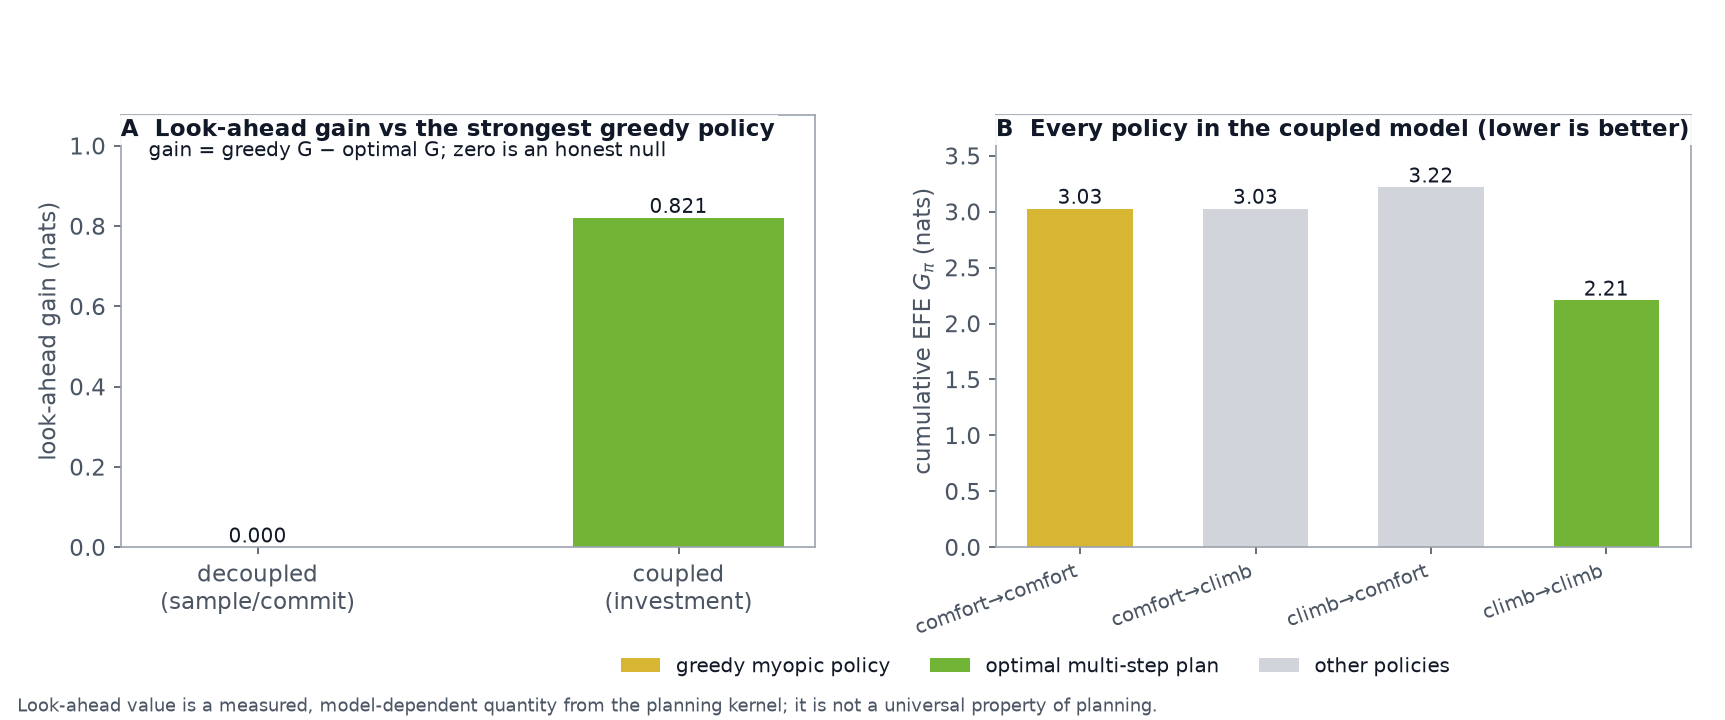
\includegraphics[width=1\linewidth,height=0.40\textheight,keepaspectratio,alt={Multi-step planning look-ahead, generated from the discrete active-inference planning kernel. The left panel contrasts the measured look-ahead gain (optimal multi-step plan versus the strongest greedy myopic policy) in a decoupled model, where the gain is zero, and a coupled investment model, where paying a worse first step to unlock the goal yields a positive gain. The right panel shows the cumulative expected free energy of every enumerated policy in the coupled model, with the greedy and optimal policies marked. The panel demonstrates that look-ahead value is a measured, model-dependent quantity, not a universal property of planning.}]{../figures/planning_lookahead.png}
\caption{Multi-step planning look-ahead, generated from the discrete
active-inference planning kernel. The left panel contrasts the measured
look-ahead gain (optimal multi-step plan versus the strongest greedy
myopic policy) in a decoupled model, where the gain is zero, and a
coupled investment model, where paying a worse first step to unlock the
goal yields a positive gain. The right panel shows the cumulative
expected free energy of every enumerated policy in the coupled model,
with the greedy and optimal policies marked. The panel demonstrates that
look-ahead value is a measured, model-dependent quantity, not a
universal property of planning.}\label{fig:planning_lookahead}
\end{figure}
\end{frame}

\subsection{Continuous predictive coding as model-specific
prediction-error
descent}\label{continuous-predictive-coding-as-model-specific-prediction-error-descent}

\begin{frame}[allowframebreaks]{Continuous predictive coding as
model-specific prediction-error descent}
The discrete examples above update beliefs in one shot; the
continuous-state face of the Free Energy Principle instead
\emph{settles} a latent estimate by descending the free energy along
precision-weighted prediction errors. On a single linear-Gaussian level
-- a vague unit-variance prior at zero meeting a more precise reading of
2 -- the estimate relaxes from the prior mean to 1.33333, the exact
analytic posterior mean, where the sensory prediction error (0.666667)
and the prior prediction error (1.33333) balance once each is weighted
by its precision.

\end{frame}

\begin{frame}[allowframebreaks]{Continuous predictive coding as
model-specific prediction-error descent}
fig.~\ref{fig:predictive_coding} shows the estimate converging to that
fixed point while, under the stated objective and step size used in this
simulation, the free energy decreases monotonically to its analytic
minimum. The result is exact for the linear-Gaussian case the kernel
tests pin against a closed form; it is a controlled teaching example,
not a claim that prediction-error descent is exact for nonlinear or
hierarchical models (Kalman 1960; Särkkä 2013; Buckley et al. 2017; Parr
et al. 2022; Kataoka and Doya 2026).

\end{frame}

\begin{frame}[allowframebreaks]{Continuous predictive coding as
model-specific prediction-error descent}
{\def\LTcaptype{none} % do not increment counter
\begin{longtable}[]{@{}
  >{\raggedright\arraybackslash}p{(\linewidth - 2\tabcolsep) * \real{0.5000}}
  >{\raggedright\arraybackslash}p{(\linewidth - 2\tabcolsep) * \real{0.5000}}@{}}
\toprule\noalign{}
\begin{minipage}[b]{\linewidth}\raggedright
Predictive-coding parameter
\end{minipage} & \begin{minipage}[b]{\linewidth}\raggedright
Paper value
\end{minipage} \\
\midrule\noalign{}
\endhead
Prior mean and variance & \(\mu_0=0\), \(\sigma_0^2=1\) \\
Observation and variance & \(y=2\), \(\sigma_y^2=0.5\) \\
Descent rate and steps & rate \(0.1\), maximum \(400\) steps \\
Analytic target & Gaussian posterior mean from the linear filtering
update \\
\bottomrule\noalign{}
\end{longtable}
}

\begin{figure}
\centering
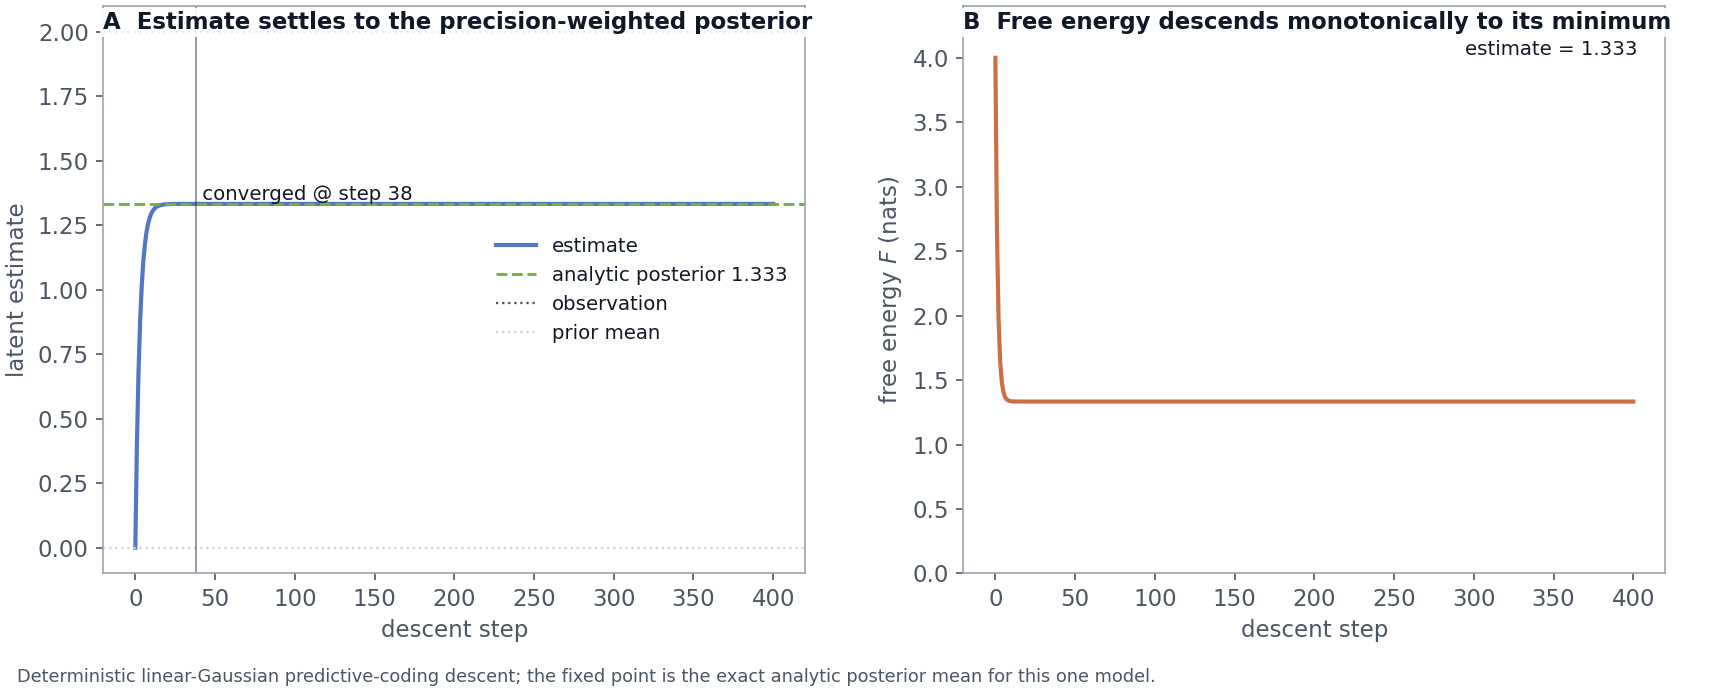
\includegraphics[width=1\linewidth,height=0.40\textheight,keepaspectratio,alt={Continuous predictive-coding descent generated from the linear-Gaussian kernel. The left panel traces the latent estimate from the prior mean to the analytic precision-weighted posterior (dashed) as it balances the sensory and prior prediction errors; the right panel shows the free energy descending monotonically to its analytic minimum. The figure supports a bounded claim that prediction-error descent implements exact Gaussian inference for this one model, not a universal convergence guarantee for all generative models.}]{../figures/predictive_coding_descent.png}
\caption{Continuous predictive-coding descent generated from the
linear-Gaussian kernel. The left panel traces the latent estimate from
the prior mean to the analytic precision-weighted posterior (dashed) as
it balances the sensory and prior prediction errors; the right panel
shows the free energy descending monotonically to its analytic minimum.
The figure supports a bounded claim that prediction-error descent
implements exact Gaussian inference for this one model, not a universal
convergence guarantee for all generative
models.}\label{fig:predictive_coding}
\end{figure}
\end{frame}

\end{document}
